\chapter{Lecture 02}

\section{Classical regularity theory for the linear problems}
We want to study the local behavior of the weak solutions \(u \in H_{loc}^{1}(\Omega; \mathbb{R}^{m})\) of a system of equations given by:
\begin{gather}
	- \sum_{\alpha, \beta, j} \partial_{x_\alpha} (A_{ij}^{\alpha \beta} \partial_{x_{\beta}} u^{j}) = f_{i} - \sum_{\alpha}^{} \partial_{x_{\alpha}} F_{i}^{\alpha}\qquad i=1,\dots,m
\end{gather}
with \(A_{ij}^{\alpha \beta} \in L^{\infty}(\Omega;\mathbb{R}), f_{i}\in L^{2}_{loc}(\Omega;\mathbb{R}), F_{i}^{\alpha}\in L_{loc}^{2}(\Omega;\mathbb{R})\).\\
In what follows we will always assume \(\Omega \subset \mathbb{R}^{m}\) to be an open, bounded and regular domain (here \(\Omega \) regular means that \(\Omega \) is locally the epigraph of a \(C^{1}\) function of \((n-1)\) variables, written in a suitable system of coordinates, near any boundary point).\\
We will see how to use a Caccioppoli-Leray inequality to prove existence of higher-order weak derivatives of \(u\) and suitable integrability results thereof. We will moreover turn such estimates into actual regularity results thanks to Sobolev embeddings. The idea above is due L. Nirenberg.\\
We use the symbol \(\vert \cdot \vert \) to denote the Hilbert-Schmidt norm of matrices and tensors, even though some estimates would be true also for the smaller operator norm.
We set
\begin{gather}
	\abs{A_{ij}^{\alpha \beta}}^{2} = \sum_{\alpha, \beta, j}  {(A_{ij}^{\alpha \beta})}^{2}
\end{gather}

\begin{thm}[Caccioppoli-Leray inequality]
	If the Borel coefficients \(A_{ij}^{\alpha \beta}\) satisfy the Legendre condition with \(\lambda>0\), namely
	\begin{gather}
		\sum_{\alpha,\beta,i,j} A_{ij}^{\alpha\beta} \xi_{\alpha}^{i} \xi_{\beta}^{j} \geq \lambda \abs{\xi}^{2}, \qquad \forall \xi \in \mathbb{R}^{m \times n}
	\end{gather}
	and
	\begin{gather}
		\sup_{x \in \Omega} \abs{A_{ij}^{\alpha\beta}(x)} \leq \Lambda < + \infty
	\end{gather}
	then there exists a positive constant \(C_{CL} = C_{CL}(\lambda, \Lambda)\) such that, for any ball \(B_{R}(x_{0})\subset \subset \Omega \) and any \(k \in \mathbb{R}^{m}\) it holds
	\begin{gather}
		C_{CL}\int\limits_{B_{\frac{R}{2}}(x_{0})}^{} \abs{\nabla u}^{2} \dd{x} \leq R^{-2}\int\limits_{B_{R}(x_{0})}^{} \abs{u(x)-k}^{2} \dd{x} + R^{2}\int\limits_{B_{R}(x_{0})} \abs{f(x)}^{2} \dd{x} +  \int\limits_{B_{R}(x_{0})} \abs{F(x)}^{2} \dd{x} \tag{CLI}\label{CLI}
	\end{gather}
\end{thm}
\begin{remark}
	\begin{itemize}
		\item the validity of~\eqref{CLI} on all \(k \in \mathbb{R}^{m}\) depends on the fact that the PDE is invariant under translation of \(u\), meaning that if \(u\) is a solution, then also \(u+k\) \(\forall k\) is a solution
		\item note also that the inequality is scale invariant: think about \(u\) being adimensional, then all the terms in~\eqref{CLI} have dimension \({(\text{length})}^{n-2}\)
		\item the inequality is surely non-trivial (the gradient of a function cannot be controlled by the variation of the function!).~\eqref{CLI} can already be regarded as a first regularity result, meaning that we are gaining specific information on the behavior of a function from the fact that it is a solution of a PDE
	\end{itemize}
\end{remark}
\begin{proof}
	W.l.o.g we take \(x_{0}=0\) and \(k=0\). We choose as test function \(\varphi \) in the weak formulation
	\begin{gather}
		\int\limits_{B_{R}}^{} \left\langle  A \nabla u, \nabla \varphi \right\rangle \dd{x} - \int\limits_{B_{R}}^{} \left\langle  f,\varphi \right\rangle \dd{x} -\int\limits_{B_{R}}^{} \left\langle  F,\nabla\varphi \right\rangle \dd{x} =0
	\end{gather}
	the function \(\varphi:= u \eta^{2}\), where \(\eta \in C_{c}^{\infty}(B_{R}; \mathbb{R})\) is a cut-off function with \(\eta \equiv 1\) in \(B_{\sfrac{R}{2}}\), \(0 \leq \eta \leq 1\) and \(\norm{\nabla \eta}_{\infty} \leq \frac{4}{R}\)
	\begin{center}
		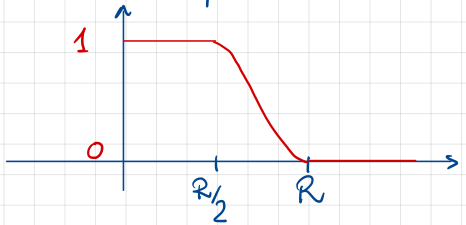
\includegraphics[scale=0.45]{pictures/picture01.png}
	\end{center}
	\begin{gather}
		\pdv[]{\varphi_{i}}{x_{\alpha}} = \pdv[]{}{x_{\alpha}} (\eta^{2}u^{2}) = \eta^{2}\pdv[]{u^{i}}{x_{\alpha}}+2 \eta \pdv[]{\eta}{x_{\alpha}} u^{i},
	\end{gather}
	that is
	\begin{gather}
		\nabla \varphi = \eta^{2} \nabla u + 2 \eta u \otimes \nabla \eta.
	\end{gather}
	Plugging in the last equality in the weak formulation
	\begin{align}
		0= & \int\limits_{B_{R}}^{} \eta^{2} \left\langle A \nabla u , \nabla u \right\rangle + 2 \int\limits_{B_{R}}^{} \eta \left\langle A \nabla u , u \otimes \nabla \eta \right\rangle  \\
		   & - \int\limits_{B_{R}}^{} \eta^{2} \left\langle f, u \right\rangle - \int\limits_{B_{R}}^{} \eta^{2} \left\langle F, \nabla u \right\rangle - 2 \int\limits_{B_{R}}^{} \eta \left\langle  F, u \otimes \nabla \eta \right\rangle  \\
		=  & : I_{1} + I_{2} -I_{3} - I_{4} - I_{5}
	\end{align}
	\begin{align}
		I_{1}:= & \int\limits_{B_{R}}^{} \eta^{2} \left\langle A \nabla u , \nabla u \right\rangle \dd{x}
		= \int\limits_{B_{R}}^{} \sum_{\alpha, \beta, i, j} \eta^{2} A_{ij}^{\alpha \beta} \partial_{x_{\alpha}} u^{i} \partial_{x_{\beta}} u^{j} \dd{x} \geq \lambda \int\limits_{B_{R}} \eta^{2} \abs{\nabla u}^{2}  \dd{x}  \\
		I_{2}:= & \, 2 \int\limits_{B_{R}}^{} \eta \left\langle A \nabla u , u \otimes \nabla \eta \right\rangle \dd{x} = 2 \int\limits_{B_{R}}^{} \eta \sum_{\alpha,\beta, i, j} A_{ij}^{\alpha \beta} \partial_{x_{\alpha}} u^{i} u^{j} \partial_{x_{\beta}} \eta \dd{x}  \\
		        & \overset{\text{Cauchy-Schwarz}}{\leq} 2 \int\limits_{B_{R}}^{} \eta \abs{A} \abs{u}\abs{\nabla u}\abs{\nabla \eta} \dd{x}  \\
		        & \overset{\text{boundedness of \(\abs{A}\) and \(\norm{\nabla \eta}_{\infty}\)}}{\leq}   \frac{( \Lambda)}{R} \int\limits_{B_{R}}^{} (\eta \abs{\nabla u}) \abs{u} \dd{x}  \\
		        & \overset{\text{Young \(ab \leq \frac{a^{2}}{2}+\frac{b^{2}}{2}\)}}{\leq} \frac{4 \Lambda}{R} \varepsilon \int\limits_{B_{R}}^{} \eta^{2} \abs{\nabla u}^{2} \dd{x} + \frac{4 \Lambda}{R \varepsilon} \int\limits_{B_{R}}^{} \abs{u}^{2} \dd{x}  \\
		I_{3}:= & \int\limits_{B_{R}}^{} \left\langle f, \eta^{2} u \right\rangle \dd{x} = \int\limits_{B_{R}}^{} \eta^{2} \sum_{i}^{} f_{i}u^{i} \dd{x}
		\overset{Young}{\leq} \frac{1}{2 R^{2}} \int\limits_{B_{R}}^{} \abs{u}^{2} \dd{x} + \frac{R^{2}}{2} \int\limits_{B_{R}}^{} \abs{f}^{2} \dd{x}  \\
		I_{4}:= & \int\limits_{B_{R}}^{} \eta^{2} \left\langle F, \nabla u \right\rangle \dd{x} = \int\limits_{B_{R}}^{} \eta^{2}\sum_{\alpha,i}^{} F_{i}^{\alpha} \partial_{x_{\alpha}} u^{i} \dd{x}
		\leq \frac{\lambda}{4} \int\limits_{B_{R}}^{} \eta^{2} \abs{\nabla u}^{2} \dd{x} + \frac{1}{\lambda} \int\limits_{B_{R}}^{} \abs{F}^{2} \dd{x}
		\intertext{By Cauchy-Schwarz inequality, \(\norm{\nabla \eta}_{\infty} \leq \frac{4}{R}\) and Young inequality we have}
		I_{5}:= & \, 2 \int\limits_{B_{R}}^{} \eta \left\langle F, u \otimes \nabla \eta \right\rangle \dd{x} = 2 \int\limits_{B_{R}}^{} \sum_{\alpha,i} F_{i}^{\alpha} u^{i} \partial_{x_{\alpha}} \eta \dd{x}
		\leq 4 \int\limits_{B_{R}}^{} \abs{F}^{2} \dd{x} + \frac{4}{R^{2}} \int\limits_{B_{R}}^{} \abs{u}^{2} \dd{x}
	\end{align}
	Therefore from the weak formulation with \( \varphi = \eta^{2} u\) we obtain
	\begin{align}
		\lambda \int\limits_{B_{R}}^{} \eta^{2}\abs{\nabla u}^{2} \dd{x}
		 & \leq \int\limits_{B_{R}}^{} \eta^{2} \left\langle A \nabla u, \nabla u \right\rangle \dd{x}  \\
		 & \leq  \underbrace{(\frac{4 \Lambda \varepsilon}{R}+ \frac{\lambda}{4}) \int\limits_{B_{R}}^{} \eta^{2}\abs{\nabla u}^{2} \dd{x}}_{\text{Dirichlet term}} + (\frac{4 \Lambda}{R \varepsilon}+\frac{1}{2 R^{2}}+\frac{4}{R^{2}}) \int\limits_{B_{R}}^{} \abs{u}^{2} \dd{x} +  \\
		 & \qquad + \frac{R^{2}}{2} \int\limits_{B_{R}}^{} \abs{f}^{2} \dd{x} + (\frac{1}{\lambda}+4) \int\limits_{B_{R}}^{} \abs{F}^{2} \dd{x}
	\end{align}
	We can choose \(\varepsilon \) so small that \(\frac{4 \Lambda \varepsilon}{R} = \frac{\lambda}{4}\) and absorb the Dirichlet term on the r.h.s.\ of the equation (meaning that it can be subtracted from both sides and still give a positive term on the left).\\
	Finally, one concludes the proof observing that
	\begin{gather}
		\int\limits_{B_{R}}^{} \eta^{2}\abs{\nabla u}^{2} \dd{x} \geq \int\limits_{B_{\frac{R}{2}}}^{} \abs{\nabla u}^{2} \dd{x}
	\end{gather}
\end{proof}
Observe that the proof shows that in \(I_{2}\) one can have a better estimate noting that \(\abs{\nabla u}=0\) on \(B_{\sfrac{R}{2}}\).
\begin{gather}
	I_{2}:= 2 \int\limits_{B_{R}}^{} \eta \abs{A} \abs{u}\abs{\nabla u}\abs{\nabla \eta} \dd{x} = 2 \int\limits_{B_{R}\setminus B_{\frac{R}{2}}}^{} \eta \abs{A}\abs{u}\abs{\nabla u}\abs{\nabla \eta} \dd{x}.
\end{gather}
This observation is indeed the starting point of the Widman's technique below.

\section{Widman ``holes filling technique''}

A sharp version of the Caccioppoli-Leray inequality~\eqref{CLI} has been proven by \underline{Widman}.\\
We can illustrate that in the simple case of \(f=0, F=0\).\\
Observe that, with the notation of the~\eqref{CLI} proof, since \(\abs{\nabla u}\leq \frac{4}{R} \chi_{B_{R}\setminus B_{\sfrac{R}{2}}}\) one obtains
\begin{gather}
	\int\limits_{B_{\frac{R}{2}}}^{} \abs{\nabla u(x)}^{2} \dd{x} leq \frac{c}{R^{2}} \int\limits_{B_{R} \setminus B_{\frac{R}{2}}}^{} \abs{u(x)-k}^{2} \dd{x} \label{001}
\end{gather}
for some positive constant \(c\) independent of \(R\).\\
Now the idea is to choose \(\kappa := \fint_{B_{R}\setminus B_{\sfrac{R}{2}}} u(x) \dd{x}\) so that we can estimate the r.h.s of~\eqref{001} using the Poincarè inequality with explicit scaling, i.e.
\begin{gather}
	\int\limits_{B_{R}\setminus B_{\frac{R}{2}}}^{} \abs{u(x)-\fint\limits_{B_{R}\setminus B_{\frac{R}{2}}}^{} u \dd{x} }^{2} \dd{x} \leq cR^{2}\int\limits_{B_{R}\setminus B_{\frac{R}{2}}}^{} \abs{\nabla u(x)}^{2} \dd{x}
\end{gather}
to get
\begin{align}
	                       & \int\limits_{B_{\frac{R}{2}}}^{} \abs{\nabla u(x)}^{2} \dd{x} \leq c \int\limits_{B_{R}\setminus B_{\frac{R}{2}}}^{} \abs{\nabla u(x)}^{2} \dd{x}  \\
	\Leftrightarrow  (c+1) & \int\limits_{B_{\frac{R}{2}}}^{} \abs{\nabla u(x)}^{2} \dd{x} \leq c \int\limits_{B_{R}}^{} \abs{\nabla u(x)}^{2} \dd{x}
\end{align}
Setting \( \vartheta := \frac{c}{c+1}<1\) we get
\begin{gather}
	\int\limits_{B_{\frac{R}{2}}}^{} \abs{\nabla u(x)}^{2} \dd{x} \leq \vartheta \int\limits_{B_{R}}^{} \abs{\nabla u(x)}^{2} \dd{x}
\end{gather}
\underline{Iterating} the previous estimates \(d\) times for radii
\begin{gather}
	2^{1}r \to 2^{2}r \to 2^{3}r \to \dots \to 2^{d}r
\end{gather}
and choosing \(r\) such that
\begin{gather}
	2^{d}r < R< 2^{d+1}r \label{002}
\end{gather}
we get
\begin{gather}
	\int\limits_{B_{R}}^{} \abs{\nabla u}^{2} \dd{x} \leq \vartheta^{d}\int\limits_{B_{R}}^{} \abs{\nabla u}^{2} \dd{x}
\end{gather}
Setting \(\alpha \log_{2}(\sfrac{1}{\vartheta})\), i.e. \(\vartheta = \sfrac{1}{2^{\alpha}}\) we have
\begin{gather}
	\vartheta^{d}= \frac{1}{2^{\alpha d}} = {\Big( \frac{1}{2^{d}} \Big)}^{\alpha} \overset{\eqref{002}}{\leq} 2^{\alpha}{\Big( \frac{r}{R} \Big)}^{\alpha}.
\end{gather}
Hence,
\begin{gather}
	\int\limits_{B_{r}}^{} \abs{\nabla u}^{2} \dd{x} \leq 2^{\alpha} {\Big( \frac{r}{R} \Big)}^{\alpha} \int\limits_{B_{R}}^{} \abs{\nabla u}^{2} \dd{x}.
\end{gather}
For \(n=2\) the estimate above implies \(u \in C^{0, \sfrac{\alpha}{2}}(\Omega; \mathbb{R}^{m})\).\\
In fact the idea that the decay of the \(L^{p}\)-norm of the gradient is related to its Hölder continuity will play a crucial role in the rest of the course, and we will discuss in detail in the next lectures.
